\section*{Spielen mit Schießpulver: \\
The Powder Toy}
\label{powdertoy}
\NewsAuthor{Horst JENS}

\textbf{Dieser Artikel beschreibt das Physik/Chemie-Simulationsspiel \textit{The Powder Toy [1]} und zeigt einen kleinen Teil der Möglichkeiten die man damit anstellen kann. 'The Powder Toy' ist freie (free/libre Open Source) Software, die von jedem Interessierten benutzt, kopiert, verändert und weiterentwickelt werden kann, gemäß den vier Grundfreiheiten welche die \textit{GPL-Lizenz [2]} gewährt.}

\begin{center}
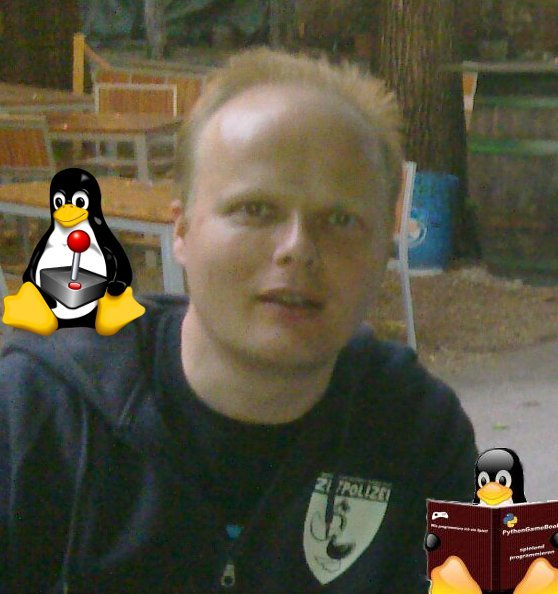
\includegraphics[width=4cm]{horst2011mitdoppeltux.jpg} \\
\footnotesize{Horst JENS. Bildrechte: [3], cc-by-sa}
\end{center}


{Hinweis:} Wenn Sie Internetverbindung haben, schauen Sie sich die folgenden Bilder online an in Farbe oder drucken Sie diesen Artikel auf einem Farbdrucker aus.

\subsection*{erst die Arbeit...}

Auf der Homepage von 'The Powder Toy' [1] kann man sich die aktuelle Version oder die noch in Entwicklung befindliche, allerneuste Beta-Version für verschiedene Betriebssysteme downloaden. Zum 'nur damit spielen' ist nichts weiter notwendig (Download starten und Spiel installieren). Weil ich vorhabe mir den \textbf{Sourcecode} genauer anschauen will habe ich mir das Programm selbst \textbf{kompiliert}. Dazu muss ich mir die tagesaktuelle Version des Programms von Github herunterladen. Wie das geht beschreibt das englische Tutorial \href{http://goo.gl/LK4z01}{\textit{Compile for Linux [4]}} im The Powder Toy Wiki ganz gut. Für Windows und Mac User gibt es im Wiki eigene Tutorials. Hier sind die Schritte die ich gemacht habe (Ubuntu Linux, 64-bit, 2 Prozessoren):

\begin{itemize}
\item Ein Terminal öffnen (Alt+STR+T) und folgendes eintippen 
\begin{center}
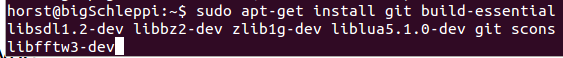
\includegraphics[width=\linewidth]{powdertoy/zeile1.png}
\end{center}
\item In jenes Verzeichnis wechseln unter welchem The Powder Toy installiert werden soll. Nachdem ich mir ein \textit{games} Verzeichnis erstellt hatte (\texttt{mkdir games}) war das bei mir das Verzeichnis \texttt{home/horst/games} deshalb musste ich dorthin wechseln mit: \texttt{cd games}  
\item Jetzt die neues Version von Github klonen (folgenden Befehl in eine einzige Zeile schreiben):
\begin{center}
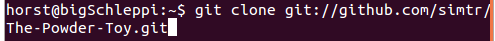
\includegraphics[width=\linewidth]{powdertoy/zeile2.png}
\end{center}
\item das Kommando \texttt{ls} (oder ein Blick auf meinen Datei-Manager) verrät mir dass ich ein neues Verzeichnis auf meiner Festplatte habe, in welches ich gleich hineinwechsle: \texttt{cd The-Powder-Game}
\item Jetzt kann der Kompiliervorgang starten! Ich tippe:
\begin{center}
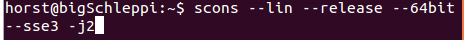
\includegraphics[width=\linewidth]{powdertoy/zeile3.png}
\end{center} Was die Parameter bedeuten wird im Wiki erklärt. Wer kein 64bit System hat lässt das \texttt{--64bit} weg, wer einen alten Computer hat lässt das \texttt{--sse3} weg und wer 4 Prozessoren hat schreibt \texttt{-j4} anstatt so wie ich \texttt{-j2} oder lässt diesen Parameter ganz weg. Nach ein paar Minuten ist das Programm fertig compiliert und befindet sich im Unterverzeichnis 'build'
\item In dieses Unterverzeichnis hineinwechseln, entweder per Dateimangaer oder per \texttt{cd build} und \texttt{ls}.
\item Je nachdem welche Parameter man gewählt hat heisst das Programm jetzt unterschiedlich. Meines heisst \texttt{powder64} und ich kann es per Doppelklick starten oder per \texttt{.\\powder64}.
\end{itemize}





